\documentclass[11pt,a4paper]{moderncv}
\moderncvtheme[blue]{classic}                
\usepackage[utf8]{inputenc}
\usepackage[top=1.2cm, bottom=1.2cm, left=1.5cm, right=1.5cm]{geometry}
\usepackage[french]{babel}
\setlength{\hintscolumnwidth}{2.9cm} % width of the left column (dates)

\firstname{Romain}
\familyname{Pellerin}
\title{Étudiant en génie informatique}    
\photo[70pt][0.0pt]{picture} % '70pt' is the height the picture must be resized to, 0.0pt is the thickness of the frame around it (put it to 0pt for no frame) and 'picture' is the name of the picture file       
\address{9 rue des réservoirs}{60200 Compiègne}    
\email{contact@romainpellerin.eu}                      
\homepage{www.romainpellerin.eu}
\mobile{07 85 25 71 64} 
\extrainfo{21 ans -- Permis B}
\quote{À la recherche d'un stage en développement logiciel}
\begin{document}
\maketitle

\section{Formation Universitaire}
\cventry{2014 -- Présent}{1\iere{} année du cycle ingénieur}{UTC (60)}{}{}{Branche Génie Informatique, formation initiale} % year, degree, institution, city+picture = {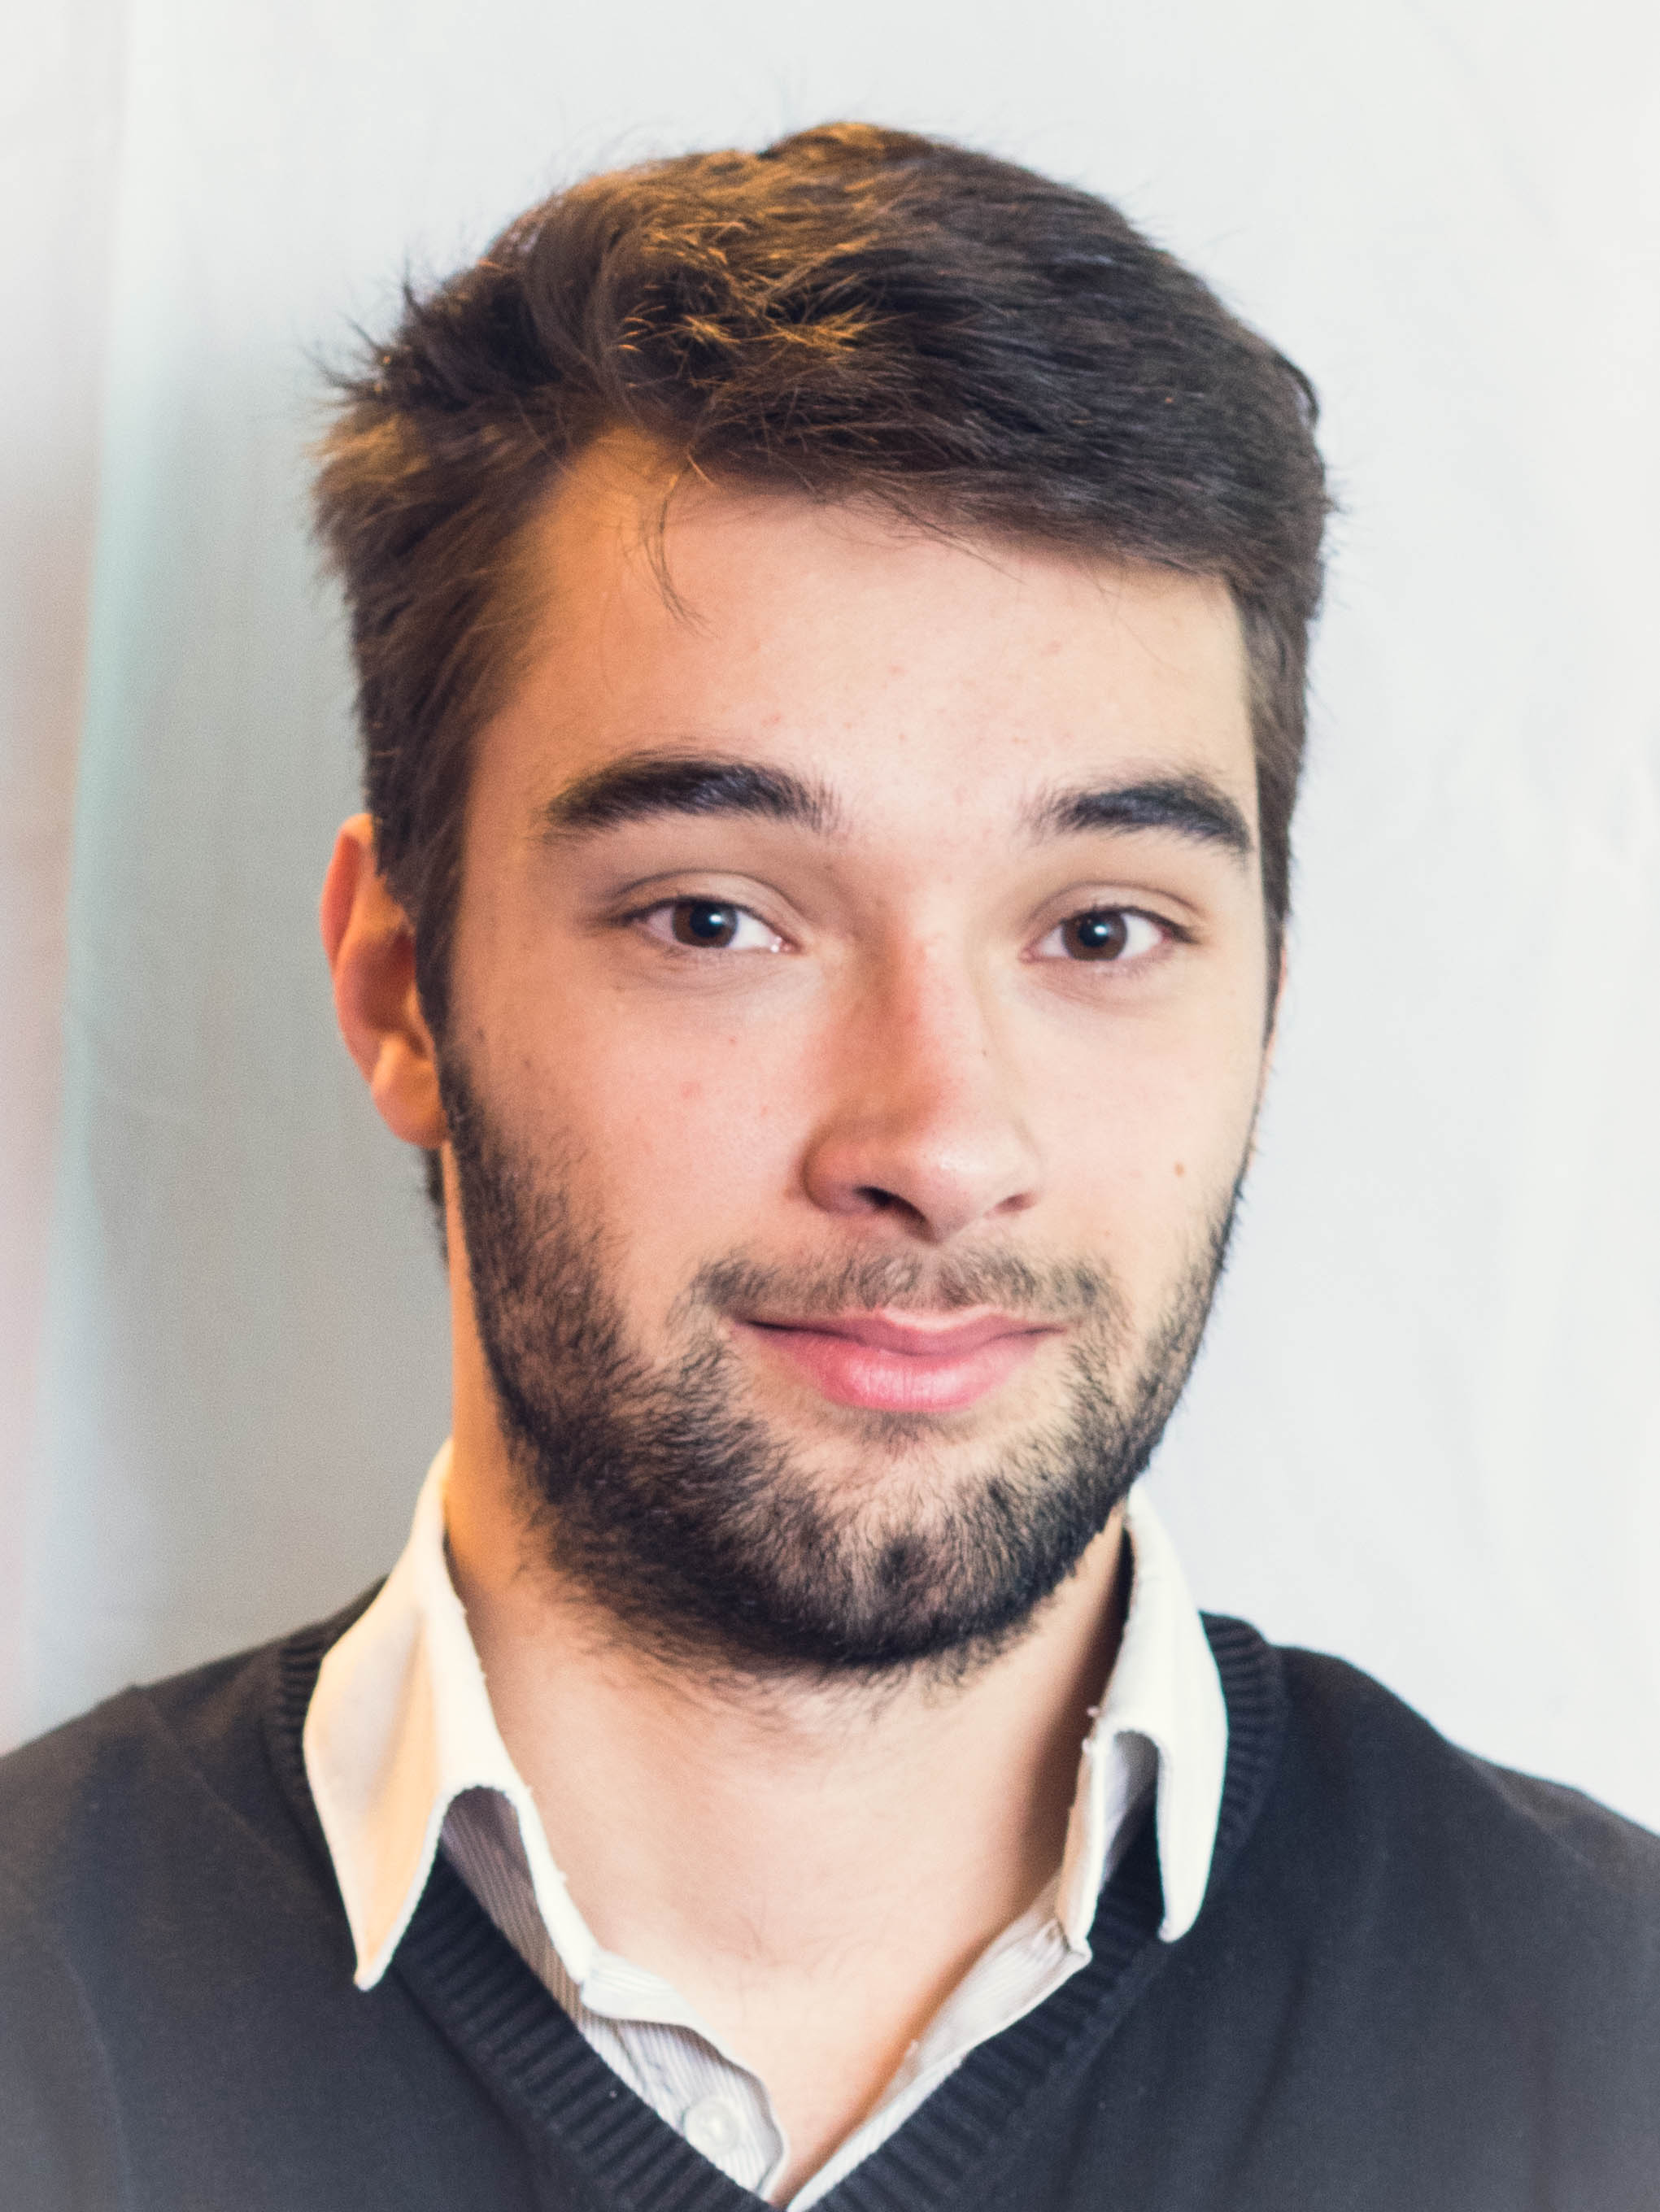
\includegraphics[scale=0.5]{picture}City}, grade, description
\cventry{2012 -- 2014}{Diplôme Universitaire de Technologie d'informatique}{IUT de Nantes (44)}{}{}{Formation initiale, 2\ieme{} de promotion}
\cventry{2011 -- 2012}{Première année de médecine}{Université de Nantes (44)}{}{}{}
\cventry{Juin 2011}{Baccalauréat Scientifique SVT spécialité mathématiques}{Lycée Jean de Lattre de Tassigny (85)}{}{}{Mention Bien}

\section{Expériences professionnelles}
\cventry{Juin 2013\\à Septembre 2014}{Auto-entrepreneur en programmation informatique}{}{Nantes}{}{Développement de l'application Android et du site web de la startup \textsc{WhoWanna}} %\newline{}

\cventry{Avril 2014\\à Juin 2014}{Stagiaire en développement logiciel}{WhoWanna}{Nantes}{}{
\begin{itemize}%
\item Migration du \textit{back-end} vers une solution de type \og\textit{cloud}\fg{}
\item Développement de la mise à jour 3.1 de l'application Android (rajout de fonctionnalités, mise à jour graphique)
\item Changement des technologies côté serveur : de PHP vers Scala et de MySQL vers PostgreSQL
\item Mise en place d'un système de \textit{versioning} (Git)
\item Rédaction d'une documentation interne à l'entreprise
\end{itemize}}

\cventry{Octobre 2013\\à Mars 2014}{Projet de deuxième année d'IUT informatique}{}{Nantes}{}{Développement d'un serveur de streaming sur un Raspberry Pi (projet de groupe), je me suis occupé du développement du serveur
(Tomcat/Java EE) et de l'application Android (Java)}

\section{Compétences en informatique}
% \cvcomputer{category}{programs}{category}{programs}
% \cvdoubleitem{subtitle}{text}{subtitle}{text}
\cvitem{Langages}{Bash, C, Java (SE et EE), PHP, HTML, CSS, Javascript, Haskell (notions), Scala (notions)}
\cvitem{Analyse}{UML, Design Patterns}
\cvitem{Bases de données}{Oracle, MySQL, Microsoft SQL Server (notions)}
\cvitem{Systèmes}{Windows XP/7/8, GNU/Linux (Debian)}
\cvitem{Administration}{Apache2, iptables, Fail2ban, OpenVPN, Git, Subversion}
%\cvitem{Logiciels}{LaTeX, Microsoft Office, LibreOffice, Adobe Photoshop}

\section{Compétences générales}
\cvitem{Anglais}{Capable de tenir une conversation, visionnage de conférences en anglais, lecture d'articles scientifiques, séries télévisées en VO -- \textbf{Toeic 895/990}} % \cvlanguage{Anglais}{}{}
\cvitem{Divers}{Notions de gestion et de communication}

\section{Centres d'intérêt}
Amateur de musique (j'ai pratiqué la guitare pendant 9 ans), je fais également du sport en loisir (course, badminton). J'aime découvrir de nouveaux langages informatiques et partager mes connaissances, j'assiste régulièrement à des conférences (DevFest, Web2Day). Je suis un fervent défenseur du logiciel libre.
\end{document}
